\documentclass[12pt,a4paper]{article}
\usepackage[utf8]{inputenc}
\usepackage{polski}
\usepackage{graphicx}

\title{Widget do monitorowania stanu urządzeń}
\author{Grzegorz Kowalski\\\texttt{daneos@daneos.com}}
\date{\today}

\begin{document}
\maketitle

\begin{abstract}
Widget pobiera dane z usługi REST, a następnie przedstawia je w formie tabelki HTML. Nazwę urządzenia podaje się jako część adresu URL. Widget aktualizuje dane co 5s używając technologii AJAX.
\end{abstract}

Widget przedstwawia dane urządzenia jako tabelkę HTML, używając opisu parametru jako tooltipu.\\
\begin{center}
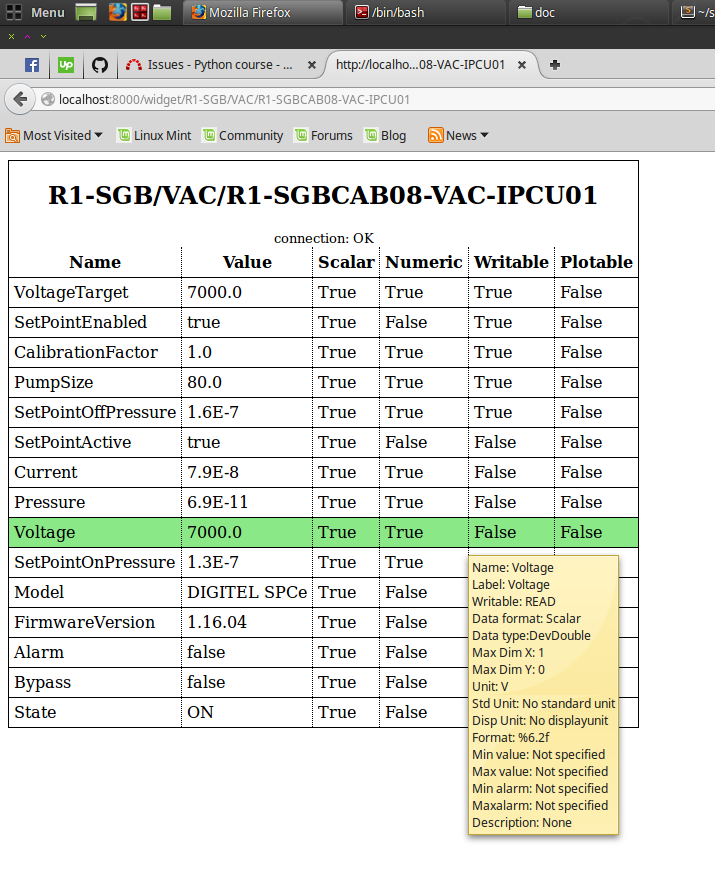
\includegraphics[width=0.6\textwidth]{./widget1.png}
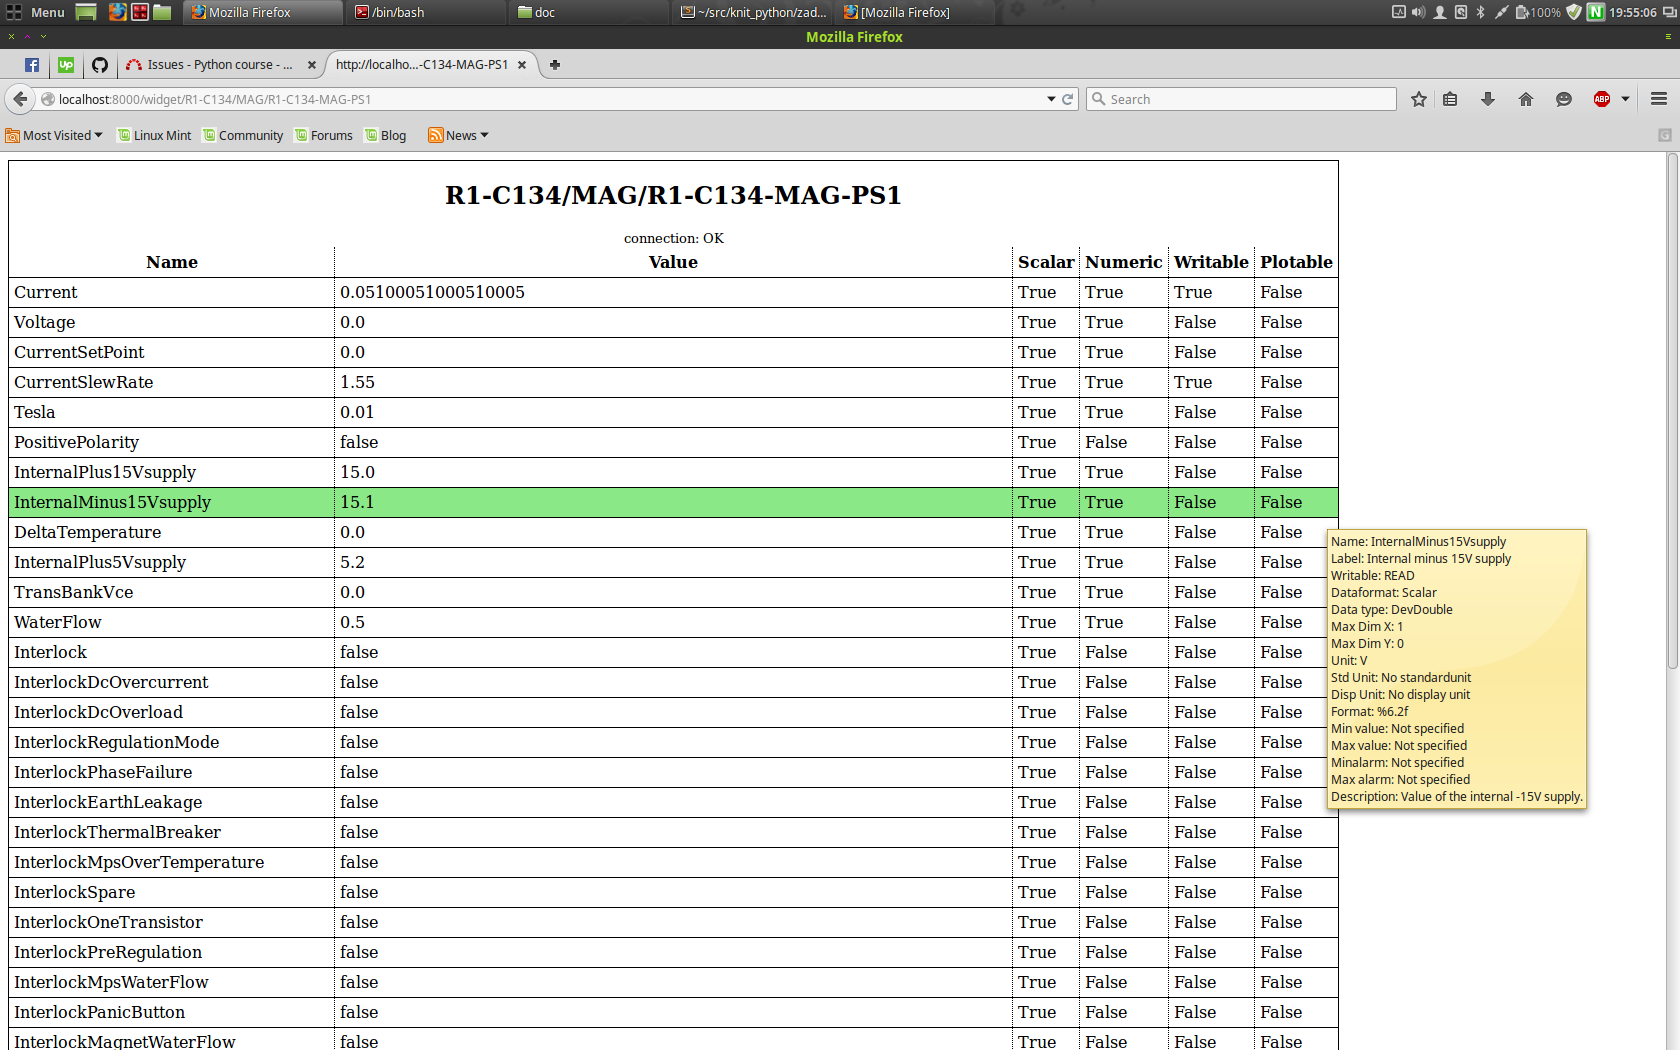
\includegraphics[width=\textwidth]{./widget2.png}
\end{center}
Aktualizacja widgetu odbywa się przez AJAX, jednak jeśli ta technologia z jakiegoś powodu nie jest dostępna, widget wyświetli odpowiednią informację.
\begin{center}
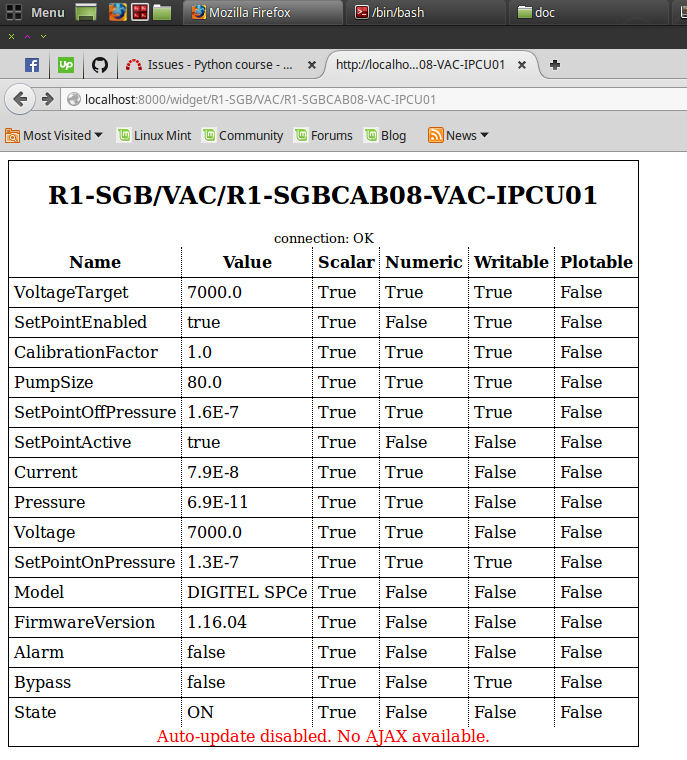
\includegraphics[width=0.7\textwidth]{./no_ajax.png}
\end{center}

\end{document}